In this section, I present the performed study using \sgp{} (\SGP) as a benchmark. The \commstr{} analyzed here consists in applying a mechanism of cost descending acceleration, exchanging the current configuration between two solvers with different characteristics. Final obtained results show that this \commstr{} works well for this problem.

\subsection{Problem definition}

The \sgp{} (\SGP) consists in scheduling $g\times p$ golfers into $g$ groups of $p$ players every week for $w$ weeks, such that two players play in the same group at most once. An instance of this problem can be represented by the triple $g-p-w$. This problem, and other closely related problems, arise in many practical applications such as encoding, encryption, and covering problems~\cite{Lardeux2014}. 

Its structure is very attractive, because it is very similar to other problems. \new{For example, the \textit{Kirkman's Schoolgirl Problem} has almost the same formulation, where a number $n$ of girls (analogous to the total number of players) walk in rows of 3 girls (analogous to the number of players per group) with the requirement that no pair of girls walk in the same row twice. An other example is the \textit{Sports Tournament Scheduling} which has a similar structure of the solution, where the number of players per group is 2, and the goal is to schedule a tournament of $n$ players over $n-1$ weeks.} %, so efficient modules to solve a broad range of problems can be built.

\new{As it was explained in Chapter~\ref{chap:art}, all benchmarks in this chapter were modeled as unconstrained optimization problems, where the objective functions is a linear combination of penalty functions associated to each constraint. The proposed model of \SGP{} has $g\times p\times w$ variables: $\left\{v_1, v_2, \dots, v_{g\times p\times w}\right\}$. Their domains are the same: $D_{v_i}=\left\{1, \dots, p\times g\right\}$.}

The cost function \new{(objective function to be minimized) for this benchmark assumes the following structure of a configuration: $s=\left(W_1, W_2, \dots, W_w\right)$, where $W_i$ are integer vectors of size $p\times g$.}

\new{This function assume that each vector $W_i$ has the structure $W_i = \left(G_1^i, G_2^i, \dots, G_g^i\right)$, where $G_j^i$ are vectors of size $p$. Based on this structure, the cost $c_s$ of a configuration is: }
\begin{equation}\label{func:cost_sgp}
c_s=\sum{}{}{\max\left(0,\left|G_i^k \cap G_j^l\right|-1\right), \forall~i,j \in [1\dots g] \text{ and } \forall~k,l \in [1\dots w], k\neq l}
\end{equation}

\new{The cost $c_s$ is penalized if some vector $W_i$ does not have its values all different.}

\poslexample{For example, let the instace 3--3--2 of \SGP{}, and a configuration $$s=\left\{1, 2, 3, 4, 5, 6, 7, 8, 9, 1, 4, 7, 2, 5, 6, 3, 8, 9\right\}$$ be. The structure of this configuration is the following:
\begin{align*}
s=&\left\{\overbrace{G_1^1, G_2^1, G_3^1}^{W_1}, \overbrace{G_1^2, G_2^2, G_3^2}^{W_2}\right\}\\
s=&\left\{\overbrace{1, 2, 3}^{G_1^1}, \overbrace{4, 5, 6}^{G_2^1}, \overbrace{7, 8, 9}^{G_3^1}, \overbrace{1, 4, 7}^{G_1^2}, \overbrace{2, 5, 6}^{G_2^2}, \overbrace{3, 8, 9}^{G_3^2}\right\}
\end{align*}
If we use the cost function defined in (\ref{func:cost_sgp}), it is clear to see that the cost $c_s = 2$.
}

The cost function for this problem was implemented making an efficient use of the stored information about the cost of the previews configuration. Using integers to work with bit-flags \new{(i.e. using integer's bits to represent boolean values)}, a table to store the partners of each player in each week can be filled in $O\left(p^2\cdot g \cdot w\right)$. So, if a configuration has $n = (p\cdot g \cdot w)$ elements, this table can be filled in $O\left(p\cdot n\right)$. This table is filled from scratch only one time in the search process (I explain in the next section why). Then, every cost of a new configuration is calculated based on this information and the performed changes between the new configuration and the stored one. This relative cost is calculated in $O\left(c\cdot g\right)$, where $c$ is the number of performed changed in the new configuration with respect to the stored one.

\subsection{Experiments design and results}

Here, I present the \as{} designed for this problem as well as concrete \oms{} composing the different solvers I have tested:

\begin{enumerate}
	\item Generation abstract module $I$:
	\subitem $I_{BP}$: Returns a random configuration $s$, respecting the structure of the problem, {\it i.e.}, the configuration is a set of $w$ permutations of the vector $[1..P]$, where $P=g\times p$.
	\item Neighborhood abstract modules $V$:
	\subitem $V_{std}$: Given a configuration, returns the neighborhood $\mathcal{V}\left(s\right)$ swapping players among groups \new{in the same week, i.e. performs all possible swaps between players in $G_i^k$ and $G_j^k$ for all $i, j \in [1...g]$ with $i < j$, and for all $k\in [1..w]$}.
	\subitem $V_{BAS}$: Given a configuration, returns the neighborhood $\mathcal{V}\left(s\right)$ swapping the most \textit{culprit player} with other players from the same week \new{but in different groups. It means that if a variable $v_i$ is selected as a culprit player and we said that for each week, it belongs to the group $\in G_{i}^k$, then $V_{BAS}$ performs all possible swaps between the player $v_i$ and all players in $G_j^k$ for all $j \in [1...g]$ with $i \neq j$, and for all $k\in [1..w]$. If a variable share the same group with another more than once, it is called a culprit player. A variable is more culprit than other, if it shares the same group with more variables than the other.} %It is based on the {\it Adaptive Search} algorithm.
	\subitem $V_{BP}(w)$: \new{Given a configuration, selects a set of $w$ weeks randomly, and returns the neighborhood $\mathcal{V}\left(s\right)$ by swapping the most culprit player with other players in the same week, for all selected weeks.} %among weeks independently selected under certain probability $p$.
	\item Selection abstract modules $S$:
	\subitem $S_{first}$: Given a neighborhood, selects the first configuration $s' \in V\left(s\right)$ improving the current cost and returns it together with the current one into the pair $\left(s', s\right)$. \new{These two configurations are returned together in order to separate two concepts: selecting a configuration to be the current one in the next iteration, and accepting it. If there is not configurations improving the cost, the first found configuration with the same cost is returned.}
	\subitem $S_{best}$: Given a neighborhood, selects the best configuration $s' \in V\left(s\right)$ improving the current cost and returns it together with the current one into the pair $\left(s', s\right)$. \new{If there is not configurations improving the cost, the first found configuration with the same cost is returned.}
	\subitem $S_{rand}$: Given a neighborhood, selects randomly a configuration $s' \in V\left(s\right)$ and returns it together with the current one, into the pair $\left(s', s\right)$.
	\item Acceptance abstract module $A$:
	\subitem $A_{AI}$: Given a pair $\left(s', s\right)$, returns always the configuration $s'$
\end{enumerate}

These concrete modules can be \new{directicly} reused to solve tournament-like problems like \textit{Sports Tournament Scheduling} and the \textit{Kirkman's Schoolgirl}, \new{because they are problems that can be modeled the same way as \SGP}.

In a first stage of the experiments, I use the operator-based language provided by \posl{} to build and test many different non-communicating strategies. The goal is to select the best concrete modules to run tests performing communication. A very first experiment was performed to select the best neighborhood function to solve the problem, comparing a basic solver using $V_{std}$; a new solver using $V_{BAS}$; and a combination of $V_{std}$ and $V_{BAS}$ by applying the operator $\circled{$\rho$}$, already introduced in the previous chapter. Algorithms~\ref{as:golfers10-10-3} and \ref{as:golfers_rho} present solvers for each case, respectively. In these algorithms, $K_1$ represents the maximum number of {\it restarts}, and $K_2$ the maximum number of iterations in each \textit{restart}.

\begin{algorithm}[t]
\dontprintsemicolon
\SetNoline
\SetKwProg{myproc}{\tet{\bf abstract solver}}{\tet{\bf begin}}{\tet{\bf end}}
\myproc{as\_simple \tcp*{{\sc Itr} $\rightarrow$ number of iterations}
	\tet{\bf computation} : $I, V, S, A$\;}{
	\whileinline{$\left(\textbf{\Iter < } K_1\right)$}{%M_1^a \circled{$\rho$} M_1^b
		$I \poslop{\mapsto}$
		\whileinline{$\left(\textbf{\Iter \% } K_2\right)$}{$\left[V \poslop{\mapsto} S \poslop{\mapsto} A\right]$}
	}	
}
\tet{\bf solver} \solverposl{Std} \tet{\bf implements} as\_simple\;
\algoindent \tet{\bf computation} : $I_{BP}, V_{std}, S_{best}, A_{AI}$ \;
\tet{\bf solver} \solverposl{AS} \tet{\bf implements} as\_simple\;
\algoindent \tet{\bf computation} : $I_{BP}, V_{BAS}, S_{best}, A_{AI}$ \; 
%\tet{\bf connection}: $CM_{last}$\;
\caption{Simple solvers for \SGP}\label{as:golfers10-10-3}
\end{algorithm}

\begin{algorithm}[H]
\dontprintsemicolon
\SetNoline
\SetKwProg{myproc}{\tet{\bf abstract solver}}{\tet{\bf begin}}{\tet{\bf end}}
\myproc{as\_rho \tcp*{{\sc Itr} $\rightarrow$ number of iterations}
	\tet{\bf computation} : $I, V_1, V_2, S, A$\;}{
	\whileinline{$\left(\textbf{\Iter < } K_1\right)$}{%M_1^a \circled{$\rho$} M_1^b
		$I \poslop{\mapsto}$
		\whileinline{$\left(\textbf{\Iter \% } K_2\right)$}{$\left[\left[V_1 \poslop{\rho} V_2\right] \poslop{\mapsto} S \poslop{\mapsto} A\right]$}
	}	
}
\tet{\bf solver} \solverposl{rho} \tet{\bf implements} as\_rho\;
\algoindent \tet{\bf computation} : $I_{BP}, V_{std}, V_{BAS}, S_{best}, A_{AI}$ \;
\caption{Solvers combining neighborhood functions using operator {\it RHO}}\label{as:golfers_rho}
\end{algorithm}

\begin{table}
\centering 
\renewcommand{\arraystretch}{1}
\begin{tabular}{p{4cm}|R{1.3cm}R{1.3cm}R{1.3cm}R{1.3cm}}
\hline
{\bf Solver} & T & T(sd) & It. & It.(sd) \\
\hline
%\hline
\texttt{\solverposl{AS}} & \good{\bf 1.06} & 0.79 & 352 & 268 \\		
\texttt{\solverposl{rho}} & 41.53 & 26.00 & 147 & 72\\
%Std $\circled{$\cup$}$ AS & 59.65 & 55.01 & 198 & 110\\
\texttt{\solverposl{Std}} & 87.90 & 41.96 & 146 & 58 \\
\hline
\end{tabular}
\caption{\sg: Instance 10--10--3 in parallel}
\label{tab:golfers10-10-3}
\end{table}

\new{Results in Table~\ref{tab:golfers10-10-3} are easy to interpret. $V_{Std}$ uses no additional information to build the neighborhood. It performs every possible swap between two players in different groups, every week, so it allows a more complete and organized search because the set of neighbors is ``pseudo-deterministic'', i.e. the construction criteria is always the same but the order in which configurations are stored is random. 
On the other hand, the neighborhood module $V_{BAS}$ selects the most culprit variable (i.e., a player), that is, the variable the most responsible for constraints violation, and permutes this variable value with the value of each other variable, in all groups and all weeks. The most culprit player is calculated as the player which has played with more other players more than once.
%with more illegal partners. A player $v_j$ is an illegal partner of the player $v_i$ if 
%Each permutation gives a neighbor of the current configuration. 
This neighborhood is $g\times p$ times smaller than the previous one, with $g$ the number of groups and $p$ the number of players per group, and their elements are more promising configurations, for that reason is more efficient, but its size make the whole search process to perform more iterations. Furthermore, it is based on the {\it Adaptive Search} algorithm, which has shown very good results \cite{Diaz}. %It selects the variable (player) contributing the most to the cost and permutes its value with the others variables (players) for all groups, every week.
$V_{BAS}$ neighborhood function takes random decisions more frequently (e.g. if there are more than one \textit{most culprit player}, one is randomly selected), and the order of the configurations is random as well. 
I also tested a solver combining these modules using the $\circled{$\rho$}$ operator. This operator executes its first or second parameter depending on a given probability $\rho$. This combination spent more time searching the best configuration among the neighborhood, although with a lower number of iterations than $V_{BAS}$. 
Since the $V_{BAS}$ neighborhood function was clearly faster, I have chosen it for our experiments, even if it shown a more spread standard deviation: 0.75 for \solverposl{AS} versus 0.62 for \solverposl{Std}, considering the ratio $\tfrac{T(sd)}{T}$.}

\separation

Once the neighborhood \om{} has been selected, I have focused the experiment on choosing the best {\it selection} \om. Solvers mentioned above were too slow to solve instances of the problem with more than three weeks: they were very often trapped into local minima. For that reason, another solver implementing the \as{} described in Algorithm~\ref{as:golfers_b001} have been created, using $V_{BAS}$ and combining $S_{best}$ and $S_{rand}$: it tries a number of times to improve the cost, and if it is not possible, it picks a random neighbor for the next iteration. We also compared the $S_{first}$ and $S_{best}$ selection modules. The \om{} $S_{best}$ selects the best configuration inside the neighborhood, so it spend more time searching a better configuration. %, but also is was more sensitive to become trapped into local minima. 
The second \om{} $S_{first}$ selects the first configuration inside the neighborhood improving the current cost. Using this module, solvers favor exploration over intensification and of course spend clearly less time searching into the neighborhood. \new{In this algorithm, $K_3$ represent the maximum number of iterations with the same current cost.}

\begin{algorithm}[H]
\dontprintsemicolon
\SetNoline
\SetKwProg{myproc}{\tet{\bf abstract solver}}{\tet{\bf begin}}{\tet{\bf end}}
\myproc{as\_eager \tcp*{{\sc Itr} $\rightarrow$ number of iterations}
	\tet{\bf computation} : $I, V, S_1, S_2, A$\tcp*{{\sc Sci} $\rightarrow$ number of iterations with the same cost}}{
	\whileinline{$\left(\textbf{\Iter < } K_1\right)$}{%M_1^a \circled{$\rho$} M_1^b
		$I \poslop{\mapsto}$
		\whileinline{$\left(\textbf{\Iter \% } K_2\right)$}{$\left[V \poslop{\mapsto} \left[S_1 \poslopcond{\Sci < K_3} S_2\right] \poslop{\mapsto} A\right]$}
	}
}
\tet{\bf solver} \solverposl{best} \tet{\bf implements} as\_eager\;
\algoindent \tet{\bf computation} : $I_{BP}, V_{std}, V_{BAS}, S_{best}, S_{rand}, A_{AI}$ \;
\tet{\bf solver} \solverposl{first} \tet{\bf implements} as\_eager\;
\algoindent \tet{\bf computation} : $I_{BP}, V_{std}, V_{BAS}, S_{first}, S_{rand}, A_{AI}$ \;
\caption{Solver for \SGP{} to scape from local minima}\label{as:golfers_b001}
\end{algorithm}

\begin{table}
\captionsetup{belowskip=6pt,aboveskip=6pt}
\centering 
\renewcommand{\arraystretch}{1}
\begin{tabular}{p{2cm}|R{1cm}R{1cm}R{1cm}R{1.2cm}|R{1cm}R{1cm}R{1cm}R{1.2cm}}
	\hline %\noalign{\smallskip}	
	\multirow{2}{*}{\footnotesize{\centering {\bf Instance}}} & 
	\multicolumn{4}{c|}{Best improvement} & 
	\multicolumn{4}{c}{First improvement}\\
	\cline{2-9} %\cline{3-8}
	& T & T(sd) & It. & It.(sd) & T & T(sd) & It. & It.(sd) \\
	\hline
	%\hline
	5--3--7 & 0.45 & 0.70 & 406 & 726 & 0.23 & 0.14 & 142 & 67\\
	8--4--7 & 0.37 & 0.11 & 68 & 13 & 0.28 & 0.07 & 93 & 13\\	
	9--4--8 & 0.87 & 0.13 & 95 & 17 & 0.60 & 0.16 & 139 & 18 \\
	\hline
\end{tabular}
\caption{\sg: comparing selection functions in parallel}
\label{tab:golfersB001}
\end{table}

\begin{table}[h]
\centering
\renewcommand{\arraystretch}{1}
\begin{tabular}{p{1.5cm}|R{1.5cm}R{1.5cm}R{1.5cm}R{1.5cm}}
\hline
{\bf Instance} & T & T(sd) & It. & It.(sd)\\
\hline
%\hline
5--3--7 & 1.25 & 1.05 & 2,907 & 2,414 \\
8--4--7 & 0.60 & 0.33 & 338 & 171 \\
9--4--8 & 1.04 & 0.72 & 346 & 193\\
\hline
\end{tabular}
\caption{\sg: a single sequential solver using first improvement}
\label{tab:golfers_seq}
\end{table}

Tables~\ref{tab:golfersB001} and \ref{tab:golfers_seq} present results of this experiment, showing that a local exploration-oriented strategy is better for the \SGP. If we compare results of Tables~\ref{tab:golfersB001} column \textit{First improvement} and \ref{tab:golfers_seq} with respect to the standard deviation, we see some gains in robustness with parallelism, using the same ratio $\tfrac{T(sd)}{T}$). \new{The reason is simple: launching a \soset{} of 40 independent solvers in parallel, is equivalent to launch 40 times a sequential solver and keep the best result}. The spread in the running times and iterations for the instance 5--3--7 is 24\% lower (0.84 sequentially versus 0.60 in parallel), for 8--4--7 is 30\% lower (0.55 sequentially versus 0.25 in parallel) and for 9--4--8 (the hardest one) is 43\% lower (0.69 sequentially versus 0.26 in parallel).

\separation

The conclusion of the last experiment was that the fastest solver to solve \SGP{} using \posl{} is the one using a neighborhood \om{} based on {\it Adaptive Search} algorithm ($V_{BAS}$) and a selection \om{} selecting the first configuration improving the cost. Using this solver as a base, the next step was to design a simple communication strategy where the shared information is the current configuration. Algorithms~\ref{as:golfers_sender}~and~\ref{as:golfers_receiver} show that the communication is performed while applying the acceptance criterion of the new configuration for the next iteration. Here, receiver solvers receive a configuration from a sender solver, match it with their current configuration, and keep the configuration with the lowest global cost. This operation is coded using the \textit{minimum} operator $\poslop{m}$ in Algorithm~\ref{as:golfers_receiver}. This way, the receiver solver continues the search from a more promising place into the search space. Different communication strategies were designed, either executing a full connected solvers set, or a tuned combination of connected and unconnected solvers. Between connected solvers, two different connections operations were applied: connecting each sender solver with one receiver solver (\oneTone), or connecting each sender solver with all receiver solvers (\oneTn). The code for the different \commstrs{} are presented in Algorithms~\ref{comm:golfers_1_1-1} to \ref{comm:golfers_1_1-n_25}. \new{In these algorithms, integer values are related to the syntactic sugar explained in Chapter~\ref{chap:posl} to declare set of solvers easy and fast.}

\begin{algorithm}
\dontprintsemicolon
\SetNoline
\SetKwProg{myproc}{\tet{\bf abstract solver}}{\tet{\bf begin}}{\tet{\bf end}}
\myproc{as\_eager\_sender \tcp*{{\sc Itr} $\rightarrow$ number of iterations}
	\tet{\bf computation} : $I, V, S_1, S_2, A$\tcp*{{\sc Sci} $\rightarrow$ number of iterations with the same cost}}{%	
	\whileinline{$\left(\textbf{\Iter < } K_1\right)$}{
		$I \poslop{\mapsto}$
		\whileinline{$\left(\textbf{\Iter \% } K_2\right)$}{$\left[V \poslop{\mapsto} \left[S_1 \poslopcond{\Sci < K_3} S_2\right] \poslop{\mapsto} \llparenthesis A \rrparenthesis^o\right]$}
	}
}
\tet{\bf solver} \solverposl{sender} \tet{\bf implements} as\_eager\_sender\;
\algoindent \tet{\bf computation} : $I_{BP}, V_{BAS}, S_{first}, S_{rand}, A_{AI}$ \;
\caption{Communicating \as{} for \SGP{} (sender)}\label{as:golfers_sender}
\end{algorithm}

\begin{algorithm}
\dontprintsemicolon
\SetNoline
\SetKwProg{myproc}{\tet{\bf abstract solver}}{\tet{\bf begin}}{\tet{\bf end}}
\myproc{as\_eager\_receiver \tcp*{{\sc Itr} $\rightarrow$ number of iterations}
	\tet{\bf computation} : $I, V, S_1, S_2, A$\tcp*{{\sc Sci} $\rightarrow$ number of iterations with the same cost}
	\tet{\bf communication} : $C.M.$\;}{%	
	\While{$\left(\textbf{\Iter < } K_1\right)$}{%M_1^a \circled{$\rho$} M_1^b
		$I \poslop{\mapsto}$
		\whileinline{$\left(\textbf{\Iter \% } K_2\right)$}{
			$ V \poslop{\mapsto} \left[S_1 \poslopcond{\Sci < K_3} S_2\right] \poslop{\mapsto} \left[A \poslop{m} C.M.\right]$
		}
	}
}
\tet{\bf solver} \solverposl{receiver} \tet{\bf implements} as\_eager\_receiver\;
\algoindent \tet{\bf computation} : $I_{BP}, V_{BAS}, S_{first}, S_{rand}, A_{AI}$ \;
\algoindent \tet{\bf communication} : $CM_{last}$
\caption{Communicating \as{} for \SGP{} (receiver)}\label{as:golfers_receiver}
\end{algorithm}

\begin{algorithm}
\dontprintsemicolon
\SetNoline
$\left[\eqsolverposl{sender}\posldot A\right] \onetoone \left[\eqsolverposl{receiver}\posldot C.M.\right]20;$
\caption{Communication strategy \oneTone{} 100\%}\label{comm:golfers_1_1-1}
\end{algorithm}

\begin{algorithm}
\dontprintsemicolon
\SetNoline
$\left[\eqsolverposl{sender}\posldot A(20)\right] \oneton \left[\eqsolverposl{receiver}\posldot C.M.(20)\right];$
\caption{Communication strategy \oneTn{} 100\%}\label{comm:golfers_1_1-n}
\end{algorithm}

\begin{algorithm}
\dontprintsemicolon
\SetNoline
$\left[\eqsolverposl{sender}\posldot A\right] \onetoone \left[\eqsolverposl{receiver}\posldot C.M.\right]10;$\;
$\left[\eqsolverposl{first}\right]20;$
\caption{Communication strategy \oneTone{} 50\%}\label{comm:golfers_1_1-1_50}
\end{algorithm}

\begin{algorithm}
\dontprintsemicolon
\SetNoline
$\left[\eqsolverposl{sender}\posldot A(10)\right] \oneton \left[\eqsolverposl{receiver}\posldot C.M.(10)\right];$\;
$\left[\eqsolverposl{first}\right]20;$
\caption{Communication strategy \oneTn{} 50\%}\label{comm:golfers_1_1-n_50}
\end{algorithm}

\begin{algorithm}
\dontprintsemicolon
\SetNoline
$\left[\eqsolverposl{sender}\posldot A\right] \onetoone \left[\eqsolverposl{receiver}\posldot C.M.\right]5;$\;
$\left[\eqsolverposl{first}\right]30;$
\caption{Communication strategy \oneTone{} 25\%}\label{comm:golfers_1_1-1_25}
\end{algorithm}

\begin{algorithm}
\dontprintsemicolon
\SetNoline
$\left[\eqsolverposl{sender}\posldot A(5)\right] \oneton \left[\eqsolverposl{receiver}\posldot C.M.(5)\right];$\;
$\left[\eqsolverposl{first}\right]30;$
\caption{Communication strategy \oneTn{} 25\%}\label{comm:golfers_1_1-n_25}
\end{algorithm}

In Algorithm~\ref{as:golfers_receiver}, the abstract \opch{} $C.M.$ was instantiated with the concrete \opch{} $CM_{last}$, which takes into account the last received configuration at the time of its execution.

Each time a \posl{} meta-solver is launched, many independent search solvers are executed. We call "good" configuration a configuration with the lowest cost within the current configuration neighborhood and with a cost strictly lesser than the current one. Once a good configuration is found in a sender solver, it is transmitted to a receiver. At this moment, if the information is accepted by the receiver, there are some solvers searching in the same subset of the search space (i.e. they continues the search from the same configuration), and the search process becomes more exploitation--oriented. This can be problematic if this process makes solvers converging too often towards local minima. In that case, we waste more than one solver trapped into a local minima: we waste all solvers that have been attracted to this part of the search space because of communications. This phenomenon is avoided through a simple (but effective) play: if a solver is not able to find a better configuration inside the neighborhood (executing $S_{first}$), it selects a random one at the next iteration (executing $S_{rand}$).

After the selection of the proper modules to study different communication strategies, I proceeded to tune parameters $K_1, K_2$ and $K_3$. Only a few runs were necessaries to conclude that the mechanism of using the \om{} $S_{rand}$ to escape from local minima was enough. For that reason, since the solver never perform restarts, the parameter $K_1$ was irrelevant. So the reader can assume $K_1 = 1$ for every experiment. With the certainty that solvers do not performs restarts during the search process, I selected the same value for $K_2 = 5000$ in order to be able to use the same \as{} for all instances. This value was selected after an experimental estimation of the upper bound of the number of iterations for the more complex instance (9--4--8). Finally, in the tuning process of $K_3$, I notice only slightly differences between using the values $5$, $10$, and $15$. So I decided to use $K_3 = 5$. \new{In this version of \posl{}, each time that we have to use different values for $K_i$ we have to change the \as. One of the goals for the next version is to include these values as parameters of the solver, in order to be even more modular.}

\begin{table}
	\captionsetup{belowskip=6pt,aboveskip=6pt}
	\centering 
	\renewcommand{\arraystretch}{1}
		\begin{tabular}{p{2cm}|R{1cm}R{1cm}R{1cm}R{1.2cm}|R{1cm}R{1cm}R{1cm}R{1.2cm}}
			\hline 	
			\multirow{2}{*}{\centering {\bf Instance}} & \multicolumn{4}{c}{Communication 1 to 1} & \multicolumn{4}{c}{Communication 1 to N}\\
			\cline{2-9}
			& T & T(sd) & It. & It.(sd) & T & T(sd) & It. & It.(sd) \\
			\hline
			%\hline
			5--3--7 & 0.20 & 0.20 & 165 & 110 & 0.20 & 0.17 & 144 & 108\\
			8--4--7 & 0.27 & 0.09 & 88 & 28 & 0.24 & 0.05 & 95 & 12\\
			9--4--8 & 0.52 & 0.14 & 117 & 25 & 0.55 & 0.14 & 126 & 20\\
%			11--7--5 & 1.76 & 0.41 & 214 & 44 & \good{1.62} & 0.34 & \good{202} & 30\\
			\hline
		\end{tabular}
	\caption{\sg: 100\% of communicating solvers}
	\label{tab:golfersB001comm100}
\end{table}

\begin{table}
	\captionsetup{belowskip=6pt,aboveskip=6pt}
	\centering 
	\renewcommand{\arraystretch}{1}
		\begin{tabular}{p{2cm}|R{1cm}R{1cm}R{1cm}R{1.2cm}|R{1cm}R{1cm}R{1cm}R{1.2cm}}
			\hline 	
			\multirow{2}{*}{\centering {\bf Instance}} & \multicolumn{4}{c}{Communication 1 to 1} & \multicolumn{4}{c}{Communication 1 to N}\\
			\cline{2-9}
			& T & T(sd) & It. & It.(sd) & T & T(sd) & It. & It.(sd) \\
			\hline
			%\hline
			5--3--7 & 0.18 & 0.13 & 125 & 88 & 0.17 & 0.12 & 139 & 81\\
			8--4--7 & 0.21 & 0.06 & 89 & 18 & 0.22 & 0.06 & 90 & 20\\
			9--4--8 & 0.49 & 0.11 & 119 & 24 & 0.51 & 0.15 & 124 & 21 \\
%			11--7--5 & 1.81 & 0.40 & 220 & 33 & 1.82 & 0.39 & 222 & 39\\
			\hline
		\end{tabular}
	\caption{\sg: 50\% of communicating solvers}
	\label{tab:golfersB001comm50}
\end{table}

\begin{table}
	\captionsetup{belowskip=6pt,aboveskip=6pt}
	\centering 
	\renewcommand{\arraystretch}{1}
		\begin{tabular}{p{2cm}|R{1cm}R{1cm}R{1cm}R{1.2cm}|R{1cm}R{1cm}R{1cm}R{1.2cm}}
			\hline 	
			\multirow{2}{*}{\centering {\bf Instance}} & \multicolumn{4}{c}{Communication 1 to 1} & \multicolumn{4}{c}{Communication 1 to N}\\
			\cline{2-9}
			& T & T(sd) & It. & It.(sd) & T & T(sd) & It. & It.(sd) \\
			\hline
			%\hline
			5--3--7 & 0.22 & 0.20 & 181 & 130 & 0.23 & 0.16 & 143 & 80\\
			8--4--7 & 0.24 & 0.08 & 95 & 22 & 0.29 & 0.09 & 93 & 12\\
			9--4--8 & 0.55 & 0.14 & 134 & 21 & 0.55 & 0.11 & 130 & 20\\
%			11--7--5 & 1.99 & 0.54 & 242 & 51 & 1.63 & 0.35 & 224 & 28 \\
			\hline
		\end{tabular}
	\caption{\sg: 25\% of communicating solvers}
	\label{tab:golfersB001comm25}
\end{table}

This communication strategy produces some gain in terms of runtime (Table~\ref{tab:golfersB001} with respect to Tables~\ref{tab:golfersB001comm100}, \ref{tab:golfersB001comm50} and \ref{tab:golfersB001comm25}). 
Having many solvers searching in different places of the search space, the probability that one of them reaches a promising place is higher. Then, when a solver finds a good configuration, it can be communicated, and receiving the help of one or more solvers in order to find the solution.
Using this strategy, the spread ratio in the running times and iterations \new{calculated from values in Table~\ref{tab:golfersB001}} was reduced for the instance 9--4--8 (0.22 using communication \oneTone{} and 50\% of communication solvers, versus 0.26), but not for instances 5--3--7 and 8--4--7 (0.70 using communication \oneTn{} and 50\% of communicating solvers versus 0.60, and 0.28 using communication \oneTone{} and 50\% of communicating solvers versus 0.25, respectively).

%Other two strategies were analyzed in the resolution of this problem, with no success, both based on the sub-division of the work by weeks, i.e., solvers trying to improve a configuration only working with one or some weeks. These strategies are:

Another \commstr{} was analyzed in the resolution of this problem, with no success, based on the sub-division of the work by weeks, i.e., solvers trying to improve a configuration only working with one week. I called \textit{Circular strategy}  and it consists in having $K$ solvers trying to improve a configuration during a given number of iteration, only working on one week. When no improvement is obtained, the current configuration is communicated to the next solver (circularly), which tries to do the same working on the next week (see Figure~\ref{subfig:golfers_bad_ring}).
This strategy did not show better results than previews strategies: \new{more than two time worse than sequential results, for every instance}. The reason is because, although the communication in \posl{} is asynchronous, most of the times solvers were trapped waiting for a configuration coming from its neighbor solver.

\begin{figure}[h]
\centering
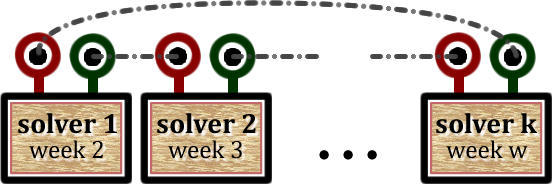
\includegraphics[width=0.45\linewidth]{golfers_ring.png}	
\caption[]{Unsuccessful communication strategies to solve \SGP}
\label{subfig:golfers_bad_ring}
\end{figure}

%\begin{enumerate}[label=\Alph*]
%\item \textbf{Circular strategy:} $K$ solvers try to improve a configuration during a given number of iteration, only working on one week. When no improvement is obtained, the current configuration is communicated to the next solver (circularly), which tries to do the same working on the next week (see Figure~\ref{subfig:golfers_bad_ring}).
%\subitem This strategy did not show better results than previews strategies: \new{more than two time worse than sequential results, for eevery instance}. The reason is because, although the communication in \posl{} is asynchronous, most of the times solvers were trapped waiting for a configuration coming from its neighbor solver.
%
%\item \textbf{Dichotomy strategy:} Solvers are divided by levels. Solvers $S_{l}^1$ in level 1 \textit{work} on one week only \new{(i.e. they use a neighborhood \om{} which generates configurations only swapping players in week $w$, with $l\in [2...w]$)}; solvers $S_{[l, l+1]}^2$ on level 2, work on 2 consecutive weeks only, and so on; and the solver $S_{[2,w]}$ on the last level ($\log_2^{w-1}+1$) that works on all weeks (except the first one). 
%Solvers in level 1 try to improve the current configuration during some number of iteration, then their best found configuration is sent to the corresponding solver: the solver on level 2 which works also with the same week. Solvers in level 2 do the same, but working on weeks $k$ to $k+1$. It means that solvers in level 2 receives configurations from the solver on level 1 working on week $k$ and from the solver on level 1 working on week $k+1$, and sends its configuration to the corresponding solver working on weeks $k$ to $k+3$; and so on. The solver in the last level works on all weeks (except the first one) and receive configuration from the solver working on weeks $2$ to $w/2$ and from the solver working on weeks $w/2+1$ to $w$ (see Figure\ref{subfig:golfers_bad_dic}). We tested this strategy with all possible levels. 
%\subitem The goal of this strategy was testing if \new{using solvers searching into small places of the focused searches rapidly communicated can help at the beginning of the search. However, the failure of this strategy come from the sent information arriving too late from the bottom to the top.
%\end{enumerate}

%\begin{figure}[h]
%	\centering
%	\subfloat[][]{
%		\label{subfig:golfers_bad_ring}
%		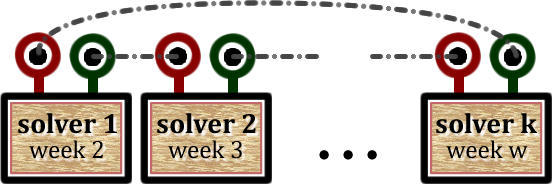
\includegraphics[width=0.45\linewidth]{golfers_ring.png}
%	} %\hspace{0.1\linewidth}
%	\subfloat[][]{%
%		\label{subfig:golfers_bad_dic}
%		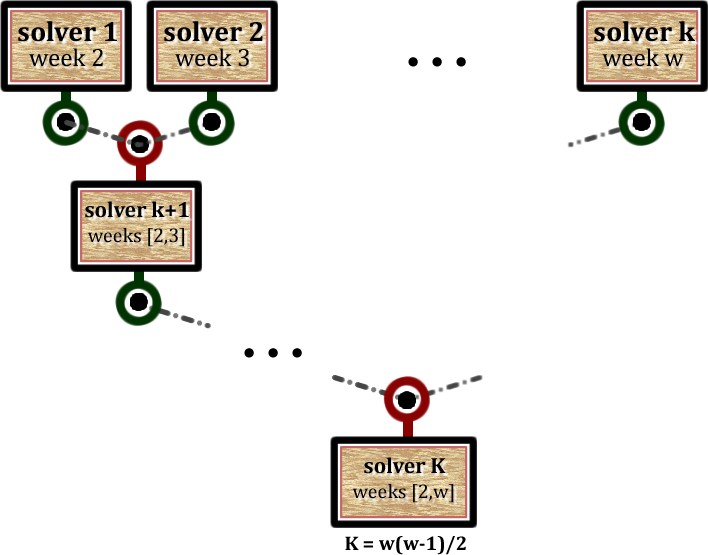
\includegraphics[width=0.45\linewidth]{golfers_dic.png}
%	}
%	\caption[]{Unsuccessful communication strategies to solve \SGP}
%	\label{fig:golfers_bad}
%\end{figure}

\separation

One last experiment using this benchmark was implementing a \commstr{} which applies a mechanism of cost descending acceleration, exchanging the current configuration between two solvers with different characteristics. Results show that this \commstr{} works pretty well for this problem.

For this strategy, new solvers were built reusing same \ms{} used for the \commstrs{} exposed before, and another different neighborhood \om{}: $V_{BP}(p)$, which given a configuration, returns the neighborhood $\mathcal{V}\left(s\right)$ by swapping the culprit player chosen for all $p$ randomly selected weeks with other players in the same week. This new solver was called \textit{companion solver}, and it descends quicker the cost of its current solution at the beginning because its neighborhood generates less values, but the convergence is slower and yet not \new{certain}. It \new{works toguether with a similar solver used for the \commstr{} exposed before}. It is called \textit{standard solver}, and converges in a stable way to the solution. So, the companion solver uses the same neighborhood function that the standard solver, but is parametrized in such a way that it builds neighbors only swapping players among two weeks.

The idea of the \commstr{} is to communicate a configuration from the companion solver to the standard solver, inn order to be able to continue the search from a more promising place into the search space. After some iterations (\new{depending on the instance}), the standard solver sends its configuration to the companion solver. The companion solver takes this received configuration and starts its search from there and finds quickly a much better configuration to send to the standard solver again. To force the companion solver to take the received configurations over its own, we use the \textit{not null} operator together with the \opch{} $C.M.$ (Algorithm~\ref{as:golfers_partial}). This process is repeated until a solution is found.

Figure~\ref{fig:solversgolfers} shows \new{a single} standard solver's run versus \new{a single} companion solver's run. In this chart we can see that, at the beginning of the run, found configurations by the companion solver have costs significantly lower than those found by the standard solver. At the 60-th millisecond the standard solver current configuration has cost 123, and the companion solver's one, 76. So for example, the communication at this time, can accelerate the process significantly.

\begin{figure}
\centering
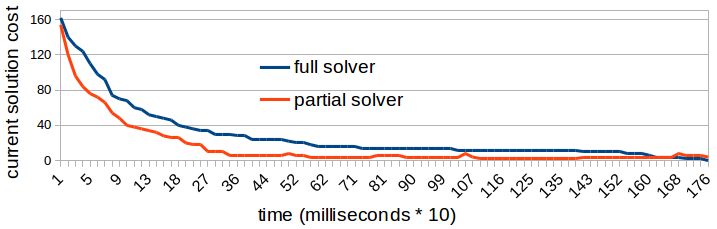
\includegraphics[width=0.9\columnwidth]{graph.png} 
\caption{Companion solver vs. standard solver (solving \sgp)}
\label{fig:solversgolfers}
\end{figure}

\begin{algorithm}
\dontprintsemicolon
\SetNoline
\SetKwProg{myproc}{\tet{\bf abstract solver}}{\tet{\bf begin}}{\tet{\bf end}}
\myproc{as\_standard \;
	\tet{\bf computation} : $I, V, S_1, S_2, A$\;
	\tet{\bf communication} : $C.M.$\;}{%
	$I \poslop{\mapsto}$
	\whileinline{$\left(\textbf{\Iter} < K_1\right)$}{
		$V \poslop{\mapsto} \left[S_1 \poslopcond{\Sci \% K_1} S_1\right] \poslop{\mapsto} \left[C.M. \poslop{m} \llparenthesis A \rrparenthesis^d\right]$		
	}
}
\tet{\bf solver} \solverposl{standard} \tet{\bf implements} as\_standard\;
\algoindent \tet{\bf computation} : $I_{BP}, V_{BAS}, S_{first}, S_{rand}, A_{AI}$ \;
\algoindent \tet{\bf communication} : $CM_{last}$ \;
\caption{Standard solver for \SGP}\label{as:golfers_full}
\end{algorithm}

\begin{algorithm}
\dontprintsemicolon
\SetNoline
\SetKwProg{myproc}{\tet{\bf abstract solver}}{\tet{\bf begin}}{\tet{\bf end}}
\myproc{as\_companion \;
	\tet{\bf computation} : $I, V, S_1, S_2, A$\;
	\tet{\bf communication} : $C.M.$\;}{
	$I \poslop{\mapsto}$
	\whileinline{$\left(\textbf{\Iter} < K_1\right)$}{
		$V \poslop{\mapsto} \left[S_1 \poslopcond{\Sci \% K_1} S_2\right] \poslop{\mapsto} \left[C.M. \poslop{\vee} \llparenthesis A \rrparenthesis^d\right]$		
	}
}
\tet{\bf solver} \solverposl{companion} \tet{\bf implements} as\_companion\;
\algoindent \tet{\bf computation} : $I_{BP}, V_{BP}(2), S_{first}, S_{rand}, A_{AI}$ \;
\algoindent \tet{\bf communication} : $CM_{last}$ \;
\caption{Companion solver for \SGP}\label{as:golfers_partial}
\end{algorithm}

We also design different \commstrs, combining connected and unconnected solvers in different percentages, and applying two different \commopers: \oneTone{} and \oneTn.

The code for the \commstr{} of 100\% of communicating solvers is presented in Algorithm~\ref{comm:golfers_v2_100} and for 50\% of communicating solvers in Algorithm~\ref{comm:golfers_v2_50}. 

\begin{algorithm}[H]
\dontprintsemicolon
\SetNoline
$\left[\eqsolverposl{companion}\posldot A\right] \onetoone \left[\eqsolverposl{standard}\posldot C.M.\right]20;$\;
$\left[\eqsolverposl{standard}\posldot A\right] \onetoone \left[\eqsolverposl{companion}\posldot C.M.\right]20;$
\caption{Companion communication strategy 100\% communication}\label{comm:golfers_v2_100}
\end{algorithm}

\begin{algorithm}[H]
\dontprintsemicolon
\SetNoline
$\left[\eqsolverposl{companion}\posldot A\right] \onetoone \left[\eqsolverposl{standard}\posldot C.M.\right]10;$\;
$\left[\eqsolverposl{standard}\posldot A\right] \onetoone \left[\eqsolverposl{companion}\posldot C.M.\right]10;$\;
$\left[\eqsolverposl{first}\right]20;$\;
\caption{Companion communication strategy 50\% communication}\label{comm:golfers_v2_50}
\end{algorithm}

This strategy produces some gain in terms of runtime as we can see in Tables~\ref{tab:golfers_v2_1N} and \ref{tab:golfers_v2_11} with respect to Table~\ref{tab:golfersB001}. It produces also more robust results in terms of runtime. The spread of results in iterations show higher variances, because there are included also results of companion solvers, which performs many times more iterations that the standard solvers. The percentage of the receiver solvers that were able to find the solution before the others did, was significant: \new{the 73\% of the receiver solvers, as a mean among the three instances, were the winners} (see Appendix~\ref{app:sgp}, Figures~\ref{barplot:5}, \ref{barplot:8} and \ref{barplot:9}), showing that the communication played an important role during the search, despite inter--process communication's overheads (reception, information interpretation, making decisions, etc).

\begin{table}
\captionsetup{belowskip=6pt,aboveskip=6pt}
\centering 
\renewcommand{\arraystretch}{1}
\resizebox{\columnwidth}{!}{%
\begin{tabular}{p{1.5cm}|R{0.8cm}R{1cm}R{0.6cm}R{1.1cm}|R{0.8cm}R{1cm}R{0.6cm}R{1.1cm}|R{0.8cm}R{1cm}R{0.6cm}R{1.1cm}}
	\hline 	
	\multirow{2}{*}{\centering {\bf Instance}} & \multicolumn{4}{c|}{Comm. \oneTn} & \multicolumn{4}{c}{(Comm. \oneTn)/2} & \multicolumn{4}{c}{(Comm. \oneTn)/4}\\
	\cline{2-13}
	& T & T(sd) & It. & It.(sd) & T & T(sd) & It. & It.(sd) & T & T(sd) & It. & It.(sd) \\
	\hline
	%\hline
	5--3--7 & 0.14 & 0.08 & 102 & 53 & 0.14 & 0.07 & 97 & 73 & 0.12 & 0.08 & 175 & 162 \\
	8--4--7 & 0.30 & 0.13 & 101 & 24 & 0.22 & 0.06 & 92 & 29 & 0.22 & 0.06 & 88 & 45 \\
	9--4--8 & 0.55 & 0.15 & 125 & 20 & 0.53 & 0.14 & 107 & 20 & 0.40 & 0.14 & 101 & 70 \\
	\hline
\end{tabular}
}
\caption{Companion \commstr{} with communication \oneTn}
\label{tab:golfers_v2_1N}
\end{table}

\begin{table}
\captionsetup{belowskip=6pt,aboveskip=6pt}
\centering 
\renewcommand{\arraystretch}{1}
\resizebox{\columnwidth}{!}{%
\begin{tabular}{p{1.5cm}|R{0.8cm}R{1cm}R{0.6cm}R{1.1cm}|R{0.8cm}R{1cm}R{0.6cm}R{1.1cm}|R{0.8cm}R{1cm}R{0.6cm}R{1.1cm}}
	\hline 	
	\multirow{2}{*}{\centering {\bf Instance}} & \multicolumn{4}{c|}{Comm. \oneTone{} (100\%)} & \multicolumn{4}{c|}{Comm. \oneTone{} (50\%)} & \multicolumn{4}{c}{Comm. \oneTone{} (25\%)}\\
	\cline{2-13}
	& T & T(sd) & It. & It.(sd) & T & T(sd) & It. & It.(sd) & T & T(sd) & It. & It.(sd) \\
	\hline
	%\hline
	5--3--7 & 0.10 & 0.05 & 98 & 75 & \good{0.08} & 0.04 & 139 & 122 & 0.11 & 0.05 & 190 & 142 \\
	8--4--7 & \good{0.14} & 0.05 & 100 & 64 & 0.22 & 0.06 & 119 & 74 & 0.21 & 0.5 & 101 & 64 \\
	9--4--8 & 0.37 & 0.14 & 86 & 65 & \good{0.36} & 0.12 & 144 & 92 & 0.45 & 0.11 & 150 & 96 \\
	\hline
\end{tabular}
}
\caption{Companion \commstr{} with communication \oneTone}
\label{tab:golfers_v2_11}
\end{table}

%This confirms the intuition that parallel approach increases the probability of finding the solution within a more reasonable time (some tens of seconds), than with the sequential scheme \cite{Alon2011}. 
%The column labeled \textbf{\% success} in Table~\ref{tab:golfers_seq} indicates the percentage of solvers finding a solution before reaching a time--out (5 minutes). 
%presented in Table~\ref{tab:golfersB001}, column \textit{O.M. First Improvement} (without communication), and results with communication (Tables~\ref{tab:golfersB001comm100}, \ref{tab:golfersB001comm50} and \ref{tab:golfersB001comm25}). 

%\subsection{Analysis of results}
%
%\modified{Then we ran experiments to study \posl's behavior solving target problems in communicating scenarios. Some compositions of solvers set were taken into account:}
%\begin{inparaenum}[i.]
%	\item the structure of the communication (with/without communication or a mix), and
%	\item \modified{the used communication operator}.
%\end{inparaenum}